%%%%%%%%%%%%%%%%%%%%%%%%%%%%%%%%%%%%%%%%%%%%%%%%%%%%%%%%%%%%%%%%%%%%%%
% LaTeX Template: Curriculum Vitae
%
% Source: http://www.howtotex.com/
% Feel free to distribute this template, but please keep the
% referal to HowToTeX.com.
% Date: July 2011
% 
%%%%%%%%%%%%%%%%%%%%%%%%%%%%%%%%%%%%%%%%%%%%%%%%%%%%%%%%%%%%%%%%%%%%%%
% How to use writeLaTeX: 
%
% You edit the source code here on the left, and the preview on the
% right shows you the result within a few seconds.
%
% Bookmark this page and share the URL with your co-authors. They can
% edit at the same time!
%
% You can upload figures, bibliographies, custom classes and
% styles using the files menu.
%
% If you're new to LaTeX, the wikibook is a great place to start:
% http://en.wikibooks.org/wiki/LaTeX
%
%%%%%%%%%%%%%%%%%%%%%%%%%%%%%%%%%%%%%%%%%%%%%%%%%%%%%%%%%%%%%%%%%%%%%%
\documentclass[paper=a4,fontsize=11pt]{article} % KOMA-article class
							
% \usepackage[english]{babel}
\usepackage[utf8x]{inputenc}
\usepackage[protrusion=true,expansion=true]{microtype}
\usepackage{amsmath,amsfonts,amsthm}     % Math packages
\usepackage{graphicx}                    % Enable pdflatex
\usepackage{hyperref}
\usepackage[svgnames]{xcolor}            % Colors by their 'svgnames'
\usepackage{geometry}
	\textheight=700px                    % Saving trees ;-)
\usepackage{url}


% \addto{\captionsenglish}{\renewcommand{\bibname}{Publications}}
% \printbibliography[title={Publications}]
\renewcommand\refname{Publications}

\frenchspacing              % Better looking spacings after periods
\pagestyle{empty}           % No pagenumbers/headers/footers

%%% Custom sectioning (sectsty package)
%%% ------------------------------------------------------------
\usepackage{sectsty}

\sectionfont{%			            % Change font of \section command
	\usefont{OT1}{phv}{b}{n}%		% bch-b-n: CharterBT-Bold font
	\sectionrule{0pt}{0pt}{-5pt}{3pt}}

%%% Macros
%%% ------------------------------------------------------------
\newlength{\spacebox}
\settowidth{\spacebox}{8888888888}			% Box to align text
\newcommand{\sepspace}{\vspace*{9pt}}		% Vertical space macro

\newcommand{\MyName}[1]{ % Name
		\Huge \usefont{OT1}{phv}{b}{n} \hfill #1
		\par \normalsize \normalfont}
		
\newcommand{\MySlogan}[1]{ % Slogan (optional)
		\large \usefont{OT1}{phv}{m}{n}\hfill \textit{#1}
		\par \normalsize \normalfont}

\newcommand{\NewPart}[1]{\section*{\uppercase{#1}}}

\newcommand{\PersonalEntry}[2]{
		\noindent\hangindent=2em\hangafter=0 % Indentation
		\parbox{\spacebox}{        % Box to align text
		\textit{#1}}		       % Entry name (birth, address, etc.)
		\hspace{1.5em} #2 \par}    % Entry value

\newcommand{\SkillsEntry}[2]{      % Same as \PersonalEntry
		\noindent\hangindent=2em\hangafter=0 % Indentation
		\parbox{\spacebox}{        % Box to align text
		\textit{#1}}			   % Entry name (birth, address, etc.)
		\hspace{1.5em} #2 \par}    % Entry value	
		
\newcommand{\EducationEntry}[4]{
		\noindent \textbf{#1} \hfill      % Study
		% \colorbox{lightgray}{%
			\parbox{12em}{%
			\hfill\color{Black}#2} \par  % Duration
		\noindent \textit{#3} \par        % School
		\noindent\hangindent=2em\hangafter=0 \small #4 % Description
		\normalsize \par}

\newcommand{\WorkEntry}[4]{				  % Same as \EducationEntry
		\noindent \textbf{#1} \hfill      % Jobname
		\colorbox{Gray}{\color{White}#2} \par  % Duration
		\noindent \textit{#3} \par              % Company
		\noindent\hangindent=2em\hangafter=0 \small #4 % Description
		\normalsize \par}

%%% ------------------------------------------------------------
\begin{document}

\nocite{*}

% you can upload a photo and include it here...
%\begin{wrapfigure}{l}{0.5\textwidth}
%	\vspace*{-2em}
%		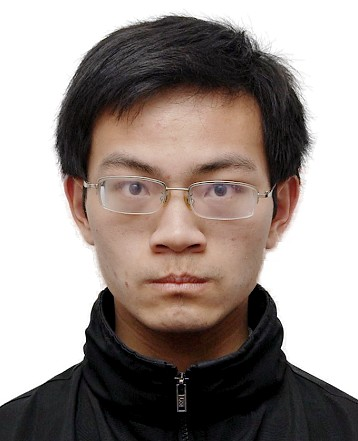
\includegraphics[width=0.15\textwidth]{photo}
%\end{wrapfigure}

\MyName{Hongxu Chen}
\MySlogan{{https://hongxuchen.github.io}}
% \MyName{Hongxu Chen~{}~}
% \MySlogan{\url{https://hongxuchen.github.io/}}


\sepspace

%%% ------------------------------------------------------------
\NewPart{Personal details}{}

% \PersonalEntry{Birth}{August 6, 1989}
\PersonalEntry{Address}{Cyber Security Lab, N4-B2C-06, NTU, Singapore}
\PersonalEntry{Phone}{+65 85476746}
\PersonalEntry{Email}{\url{hongxuchen@outlook.com}, \url{hchen017@e.ntu.edu.sg}}
\PersonalEntry{LinkedIn}{\url{https://www.linkedin.com/in/hongxu-chen-09a97640}}

%%% ------------------------------------------------------------
\NewPart{Education}{}

\EducationEntry{Ph.D in Computer Engineering}{2015.8-2019.8(expected)}{Nanyang Technological University}{
    I have been focusing on Cybersecurity research in mobile applications and software. I developed a permission-dependent security type system for enforcing information flow in Android~\cite{sta}, as well as surveyed the Android Malware~\cite{XueM0TC0Z17}. I also developed a Fuzzing Orchestration Toolkit (FOT)~\cite{fse18-fot} which detected 200+ vulnerabilities in well-known open source projects such as GNU Binutils, GNU diffutils, libjpeg, ffmpeg, among these 42 CVEs have been assigned. On top of FOT, I aslo developed a novel directed greybox fuzzing technique~\cite{hawkeye} that targets on fuzzing specific locations of the program. FOT has received the first award in the 16th National Software and Application Conference (NASAC 2017) prototype competition (fixed topic).
}
\sepspace

\EducationEntry{MSc. in Computer Science}{2011.9-2014.3}{Shanghai Jiaotong University}{
  I have been doing LLVM based static analysis for C/C++ programs, as well as SOOT based analysis for Java programs.}
\sepspace

\EducationEntry{BSc. in Mathematics}{2007.9-2011.6}{Nanjing University of Science and Technology}{}

%%% ------------------------------------------------------------
\NewPart{Work experience}{}

\EducationEntry{Research Associate}{2014.5-2015-8}{Nanyang Technological University}{
I have been involved in a symbolic analysis on C/C++ programs and developed a static bug detection tool with precise points-to analysis and loop summarization based on LLVM~\cite{XieLLLC15}.}
\sepspace

\EducationEntry{Research Intern}{2013.2-2013.11}{Microsoft Research Asia, Beijing}{
I have worked in System Research Group in Microsoft Research Asia in developing a scopped symbolic execution backed with LLVM based static program slicing and KLEE symbolic executor.}
\sepspace

%%% ------------------------------------------------------------
\NewPart{Skills}{}

\SkillsEntry{Languages}{Chinese Mandarin, English}
\SkillsEntry{Software}{{LLVM, Rust, C/C++, Java, Python}}
\SkillsEntry{}{Linux Programming, Bash, Radare2}
\SkillsEntry{}{Scala,OCaml, Haskell, Coq, Isabelle}

\pagebreak

\NewPart{Discovered Bugs}
Below are the selected bugs, vulnerabilities discovered by me; several of them have been assigned CVE IDs. Detailed information is available at \url{https://hongxuchen.github.io/}.
\begin{enumerate}
    \item binaryen: 17 bugs
    \item CImg: 2 bugs
    \item Espruino: CVE-2018-11590, CVE-2018-11591, CVE-2018-11592, CVE-2018-11593, CVE-2018-11594, CVE-2018-11595, CVE-2018-11596, CVE-2018-11597, CVE-2018-11598
    \item Exiv2: CVE-2018-19107, CVE-2018-19108, CVE-2018-19535
    \item FFmpeg: CVE-2018-15822, CVE-2018-14394, CVE-2018-14395
    \item FLIF: 2 bugs
    \item glibc and gnulib: CVE-2009-5155, CVE-2019-9169, CVE-2018-20796
    \item GNU bc: 18 bugs
    \item GNU Binutils: CVE-2018-17794
    \item GNU diffutils: 2 bugs (git fix)
    \item GNU grep: 34140
    \item GNU sed: 34141, 34142
    \item GraphicsMagick: 1 performance issue
    \item GPAC: 15 bugs
    \item JSMN: 1 bug
    \item imagemagick: CVE-2018-14560 (RESERVED), CVE-2018-14561 (RESERVED)
    \item Intel XED: 2 categories of bugs
    \item libjpeg-turbo: CVE-2018-14498
    \item libtoml: 6 bugs
    \item lepton: 4 bugs
    \item liblnk: 19 bugs (most of the root causes are inside its library libfwsi)
    \item liblouis: 1 bug(CVE-2018-17294)
    \item libmobi: 4 bugs
    \item libpff: 3 bugs
    \item libsass: 10 bugs, CVE-2018-19837, CVE-2018-19838, CVE-2018-19839,
    \item libsixel: 5 crashes and 1 performance issue
    \item libvips: 11 bugs
    \item MJS: 33 bugs
    \item mozjpeg: 1 bug
    \item mxml: CVE-2018-20592, CVE-2018-20593
    \item openh264: 1 bug
    \item poppler: CVE-2018-20662
    \item radare2: 40+ bugs, CVE-2018-19842, CVE-2018-19843, CVE-2018-20455, CVE-2018-20456, CVE-2018-20457, CVE-2018-20458, CVE-2018-20459, CVE-2018-20460, CVE-2018-20461
    \item solidity: 2 crashes and 1 performance issue
    \item Swift: 7 bugs (SR-8467, SR-8468, SR-8476, SR-8483, SR-8576, SR-8577)
    \item tinyexr: 6 bugs
    \item WAVM: 2 bugs(CVE-2018-17292, CVE-2018-17293)
    \item WavPack: CVE-2018-19840, CVE-2018-19841
    \item WebM: 1 bug
    \item xdrpp: 1 bug
    \item yaml-cpp: 2 bugs
\end{enumerate}


\bibliography{pub} 
\bibliographystyle{plain}
\end{document}
